\section{Tests}
\subsection{Zeitliche Analyse}
\subsubsection{Test Simulation mit System Viewer}
In Abb: \ref{fig4} wird eine Sequenz der Simulation während sich das Programm in einer Pause befindet, also keine Aufträge auszuführen sind, gezeigt. Diese Sequenz beginnt mit dem Beweger-Task (1.) welcher die virtuelle Position des Turms aktualisiert. Anschließend werden alle Sensor-Tasks nacheinander aktiv und überprüfen ob sich an ihrer Stelle gerade der Turm befindet und schreiben ihre Antwort darauf in die MessageQueue. Diese wird von dem Sensor-Collector, nachdem alle Sensoren durchgelaufen sind, ausgelesen und von diesem zu einem Gesamt-Konstrukt zusammengefügt und in die MessageQueue an die HRL-Steuerung geschrieben. \\
Das Gantt-Diagramm  Abb: \ref{gantt} wird damit bestätigt.

\begin{figure}[H]
	\centering
  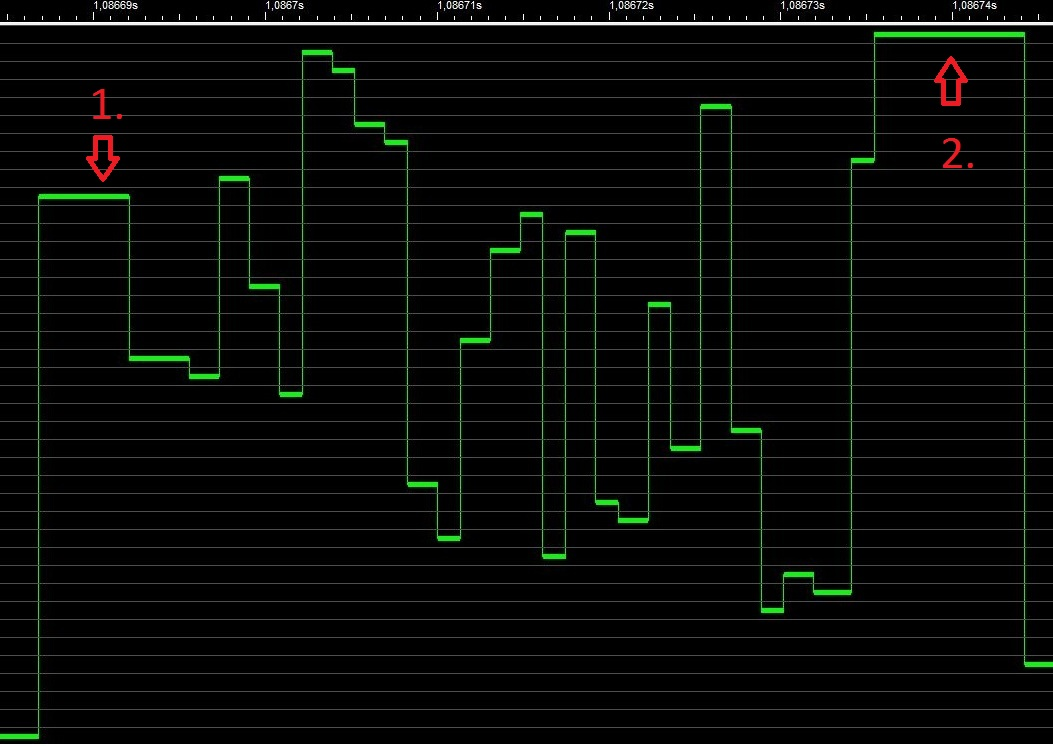
\includegraphics[width=0.8\textwidth]{diagrams/simulation_erklaerung.jpg}
	\caption{Simulation mit System Viewer}
	\label{fig4}
\end{figure}
\subsubsection{Test Hochregal-Steuerung mit System Viewer}
Die Hochregal-Steuerung besteht aus lediglich zwei Tasks, welche sich nicht unterbrechen. Der Movement-Task (1.) beginnt mit der Berechnung der Aktor-Befehle, welche anschließend von dem AktorPushData-Task(2.) an die Simulation weitergeleitet werden. Auch dieses ist somit Bestätigt.
\begin{figure}[H]
	\centering
  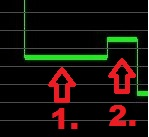
\includegraphics[width=0.4\textwidth]{diagrams/steuerung_zeit.jpg}
	\caption{HRL-Steuerung mit System Viewer}
	\label{fig5}
\end{figure}
\subsection {Systemtests}

\subsubsection {Jobannahmetest}
\begin{tabular}{|l|l|l|l|l|}
\hline
 aktuell | neu -->&  vsetspace x y & clearspace x y  & insert x y & remove x y\\
\hline
vsetspace	x y & pass & pass & pass  & pass\\
\hline
clearspace	x y & pass & pass & pass  & pass \\
\hline
insert 		x y & pass & pass & pass & pass\\
\hline
remove	x y & pass & pass & pass & pass\\
\hline
\end{tabular}
\ \\
Nach diesem Test können wir bestätigen, dass das Programm aus jedem Job in den Folgejob gelangt.

\subsubsection {Vollständigkeit / Korrektheit} 

\begin{tabular}{|l|l|}
\hline
         	& Änderung der Belegungsmatrix\\
\hline
vsetspace & pass\\
\hline
\end{tabular}

Dieser Test bestätigt die Funktion des vsetspace-Befehls innerhalb der Spezifikationen.

\begin{tabular}{|l|l|}
\hline
         	& Änderung der Belegungsmatrix\\
\hline
clearspace & pass\\
\hline
\end{tabular}

Dieser Test bestätigt die Funktion des clearspace-Befehls innerhalb der Spezifikationen.


\begin{tabular}{|l|l|l|l|l|}
\hline
         	&  fahre zur Eingabe & Paket annehmen   & fahre zur Ablage & Paket ablegen\\
\hline
insert x y & pass & pass & pass & pass\\
\hline
\end{tabular}

Dieser Test bestätigt die Funktion des insert-Befehls innerhalb der Spezifikationen.

\begin{tabular}{|l|l|l|l|l|}
\hline
         	&  fahre zur Ablage & Paket annehmen   & fahre zur Augabe & Paket ablegen\\
\hline
remove x y & pass & pass & pass & pass\\
\hline
\end{tabular}

Dieser Test bestätigt die Funktion des remove-Befehls innerhalb der Spezifikationen.\\
\\
Zudem wurde das Verhalten der automatisches Einlagerung überprüft falls das Regal voll ist. In diesem fall wird der Job nicht mehr angenommen und der zustand am Terminal ausgegeben.\\
\\
Falls mehrere Befehle in der Warteschlange den selben Platz setzen oder leeren wollen wurde dies nicht erkannt, dieses fehlverhalten wurde verbessert  und am Terminal quittiert.


\subsubsection {Test außerhalb der Spezifikationen}

In diesem Test wird das verhalten des Programmes bei Fehlbedienung getestet, ein pass bedeutet das der Job nicht angenommen wird.

\begin{tabular}{|l|l|l|l|l|}
\hline
         	&  x<0 | y<0 & x > 9 | y > 4 & ohne Param.& ende von Pause oder Zusatz\\
\hline
vsetspace & pass & pass & pass & pass \\
\hline
clearspace & pass & pass & pass & pass \\
\hline
insert & pass & pass & pass & pass \\
\hline
remove & pass & pass & pass & pass \\
\hline
\end{tabular}

Dieser Test bestätigt das bei jeder fehlerhaften Eingabe der Job nicht angenommen wird und dieses auch am Terminal anzeigt.




